\documentclass[11pt]{article}

\usepackage[a5paper,left=2cm,right=1cm,top=1cm, bottom=1.5cm]{geometry}
\usepackage{array}
\usepackage{makecell}
\usepackage[all]{nowidow}
\usepackage{wrapfig}
\usepackage{enumitem}
\usepackage{multicol}

\usepackage{hyperref}
\hypersetup{
    colorlinks=true,
    urlcolor=sokolblue,
    }

\usepackage[czech]{babel}
\usepackage[utf8]{inputenc} 
\usepackage{ellipsis}

\usepackage{fontspec}
\newfontfamily{\tyrs}{Sokol Tyrs}
\newfontfamily{\fugner}{Sokol Fugner}

% \usepackage{lmodern}
% \usepackage[T1]{fontenc} 
\usepackage{anyfontsize}
\newcommand{\titlesize}{\fontsize{56pt}{67pt}}


\usepackage[dvipsnames]{xcolor}
\definecolor{sokolred}{RGB}{228, 5, 33}
\definecolor{sokoldarkred}{RGB}{200, 0, 30}
\definecolor{sokolblue}{RGB}{45, 46, 135}

\usepackage{tikz}
\usetikzlibrary{calc}

\usepackage{fancyhdr}

\fancypagestyle{standard}{%
    \fancyhf{}
    \fancyhead[LO]{%
        \begin{tikzpicture}[overlay,remember picture]
            \fill [color=sokolred] (current page.north west) rectangle ($ (current page.south west) + (1cm,0cm) $);
            \fill [color=sokolred] ($ (current page.north west) + (1.1cm,0cm) $) rectangle ($ (current page.south west) + (1.2cm,0cm) $);
        \end{tikzpicture}
        }
    % \fancyhead[RE]{%
    %     \begin{tikzpicture}[overlay,remember picture]
    %         \fill [color=orange](current page.north east) rectangle
    %             ($ (current page.south east) + (-1cm,0cm) $);
    %     \end{tikzpicture}
    %     }
    \fancyfoot[C]{%
      \begin{tikzpicture}[overlay,remember picture]
        \fill [color=sokolred] ($ (current page.south east) + (-1.5cm,1.3cm) $) rectangle ($ (current page.south east) + (0cm,0.5cm) $)
         node [pos=0.5,color=white] {\large\tyrs{\thepage}\hspace*{0.5cm}};
      \end{tikzpicture}
    }

    \renewcommand{\headrulewidth}{0pt}
    \renewcommand{\footrulewidth}{0pt}
}



\fancypagestyle{uvodnik}{%
    \fancyhf{}
    \fancyfoot[C]{%
      \begin{tikzpicture}[overlay,remember picture]
        \fill [color=sokolred] ($ (current page.south east) + (-1.5cm,1.3cm) $) rectangle ($ (current page.south east) + (0cm,0.5cm) $)
         node [pos=0.5,color=white] {\large\tyrs{\thepage}\hspace*{0.5cm}};
      \end{tikzpicture}
    }

    \renewcommand{\headrulewidth}{0pt}
    \renewcommand{\footrulewidth}{0pt}
}

\fancypagestyle{blank}{%
    \fancyhf{}
    \fancyfoot[C]{}

    \renewcommand{\headrulewidth}{0pt}
    \renewcommand{\footrulewidth}{0pt}
}


\newcommand{\post}[1]{%
\begin{center}
{\huge \tyrs #1}
\end{center}
}

\newcommand{\subpost}[1]{%
\vspace*{12pt}
\begin{center}
{\Large \tyrs #1}
\end{center}}

\newcommand{\signature}[2]{%
  \begin{flushright}
    \textbf{#1}\\#2
  \end{flushright}
}

\newcommand{\luv}{\clqq\kern-0.07em}
\newcommand{\ruv}{\kern0.07em\crqq\kern0.1em}

\usepackage{csquotes}
\DeclareQuoteAlias{german}{czech}
\MakeOuterQuote{"}

\usepackage[normalem]{ulem}


\begin{document}

%% title
\newgeometry{margin=1cm}
\pagecolor{sokolred}
\color{white}
\pagenumbering{gobble}
\begin{center}
\vspace*{\fill}

{\titlesize \fugner ZPRÁVY}

{\titlesize \tyrs SOKOLA LIBEŇ}

\vspace*{1cm}

{\large ročník L · číslo 1 · únor 2024}

\vspace*{\fill}
\end{center}

\clearpage
\normalcolor
\nopagecolor
\pagenumbering{arabic}

%% úvodník
\pagestyle{uvodnik}
\newgeometry{margin=1.5cm}


{\fontsize{48pt}{57pt} \fugner \color{sokolred} \noindent Úvodník}
\hfill
{\textbf{br. Tomáš Dragoun}} %\raisebox{24pt}{...}

\vspace*{12pt}

\noindent
Vážení členové Sokola Libeň,

\noindent
v~čase psaní těchto Zpráv ještě nejsou nové šatny v~provozu, ale je jisté, že se otevřou/otevřely v~pondělí 19. února. Končí tak nepříliš pohodlné období, kdy se členové Sokola převlékali po celé sokolovně a i návštěvníci Sokola byli možná až moc blízko \luv{}běžnému\ruv{} životu v~sokolovně. Jak cvičencům, tak cvičitelům, doprovázejícím rodičům i dalším návštěvníkům moc děkuji, že tyto dočasné ztížené podmínky zvládli a měli pro ně pochopení. Toto poděkování je možná zbytečné, protože sokolové si v~nepohodlí libují, ale stejně děkuji.

S~tím souvisí i drobné plánované změny v~provozu nových šaten. Máme je hezky rozmyšlené a shrnuté v~provozním řádu, ale až praxe je prověří. Nemůžeme vyloučit, že pravidla používání šaten budeme ještě ladit. Prosím vás tedy o~zvýšenou pozornost, co se týče pokynů cvičitelů ohledně vstupu do šaten. Co se měnit nebude, je skutečnost, že šatny jsou nyní \luv{}čistou zónou\ruv{}, kam není možné nosit venkovní obuv. Venkovní boty zůstávají v~předsálí.

Cvičení v~oddílech je nyní velmi nabité. Nacvičují se sletové skladby, vystoupení na akademii, probíhá příprava na závody všestrannosti.

Ve Zprávách pak najdete termínovou listinu připravovaných akcí. Z~těch bych upozornil na zmíněnou akademii (sobota 2. března) a Šibřinky, rovněž v~sobotu, 23. března.

Naše jednota v~letošním roce slaví 140 let od svého založení. K~této události najdete ve Zprávách kvíz či vzpomínku na založení jednoty. Pro nás členy se jedná o~významné výročí, které bychom s~Vámi rádi na podzim náležitě oslavili. Podrobnosti oslav budeme postupně sdílet.


\clearpage

%% termínka

\pagecolor{sokolred}
\color{white}
\renewcommand{\arraystretch}{1.4}

\newcommand{\boxheight}{12.3cm}

\vspace*{\fill}
\post{TERMÍNOVÁ LISTINA AKCÍ JEDNOTY}
\vspace*{0pt}

\begin{center}
\begin{tikzpicture}
  \draw [ultra thick,color=white](0.3cm,0cm) rectangle (12.3cm,\boxheight);
  \fill [color=white] (0cm,0.3cm) rectangle (12cm,\boxheight + 0.3cm)
  node [pos=.5, color=black] {
    \begin{tabular}{l  p{6.5cm}}
      20.+22. 2. 2024 (út, čt) & Nominační závody žáků \\
      2. 3. 2024 (so) & Akademie (přesunutá z~podzimu) \\
      3. 3. 2024 (ne) & Jarní brigáda \\
      20. 3. 2024 (st) & Valná hromada jednoty \par \textit{účast zvolených delegátů nutná, další členové vítáni} \\
      23. 3. 2024 (so) & Šibřinky \par \textit{odpoledne dětské, večer dospělé}  \\
      13. 4. 2024 (so) & 66. Jarní Výlet Libeňského Sokola \\
      19.–12. 4. (pá–ne) & Župní závody všestrannosti \\
      25. 4. 2024 (čt) & Premiéra divadelní hry Sokolské peklo \\
      10.–12. 5. (pá–ne) & Republikový přebor ZZZ (Úpice, pokud někdo postoupí) \\
      25.–26. 5. (so–ne) & Oblastní Slet v~Brandýse nad Labem \\
      30. 5. 2024 & Dětský den \\
      během května & zápis do oddílu Rodičů a dětí, Předškolních dětí \\ 
      30. 6. – 5. 7. & Slet \\
      5. 7. 2024 & Posletový táborák \\
    \end{tabular}
  };
  %  node [color=black] {FOOBAR};
\end{tikzpicture}

\renewcommand{\arraystretch}{1}

\vspace*{12pt}
Sledujte naše stránky a zprávy ze systému EOS, kde budeme postupně uveřejňovat podrobnosti k~jednotlivým akcím.

\end{center}
\vspace*{\fill}

\clearpage
\nopagecolor
\normalcolor

%% normální obsah
\restoregeometry
\pagestyle{standard}

\post{140 let}

Říkáte si, co je to za číslo? Nevíte? Tak vězte, že 26. 10. 1884 byl založen Sokol v~Libni. Letos to tedy bude už 140 let od založení naší jednoty.

Pro ilustraci uvádím úryvek z~Almanachu vydaného ke 100. výročí založení jednoty v~roce 1984 (kdy jsme byli jako odbor ZRTV součástí tělovýchovné jednoty Meteor Praha):


\it
\vspace*{12pt}
\noindent\textbf{V pravdě stůj, vlast miluj, nechtěj porobu, služ vlasti, národu!}

\vspace*{12pt}
\noindent Slova chorálu v~závěru vystoupení mužského dorostu na VIII. sletu všesokolském v~roce 1926 byla již o~42 let dříve vůdčím heslem několika pokrokových a vlasteneckých občanů, jež osud zavál do tehdejší vesnice Libně, v~okresu karlínském, aby tu byli šiřiteli národní osvěty. Buďte zde pro trvalou a oživovanou paměť zachována jejich jména:

\vspace*{6pt}
\begin{itemize}[
  itemsep=-3pt,
  leftmargin=2em,
  itemindent=-1em
]
\item[] \textbf{Ladislav Verner}, nar. 7. 1. 1856 v~Byháni, učitel obecné školy chlapecké od 21. 4. 1882.
\item[] \textbf{Jaroslav Pechan}, nar. 15. 10. 1882 v~Praze, od 2. 11. 1882 zatímní podučitel do 5. 8. 1886, kdy odešel do Kozel.
\item[] \textbf{František Gliman}, nar. 6. 5. 1862 v~Chocni, dočasný smluvní učitel od 1. 9. 1882, odešel do Nehvizd 1. 3. 1886.
\item[] \textbf{Václav Kalaš}, provizorní podučitel od 2. 11. 1882, odešel do Prahy 9. 12. 1885.
\end{itemize}
\vspace*{6pt}
\noindent

Tito čtyři mladí učitelští mládenci, z~nichž Jaroslav Pechan již od roku 1880 je členem-stipendistou Sokola Pražského, a tedy pod přímým vlivem Dr. Miroslava Tyrše i jako cvičitel jeho Tělocvičného ústavu pro hochy, našli ubytování ve třech místnostech v~tzv. staré faře Dr. Košáka.

I~u~nás, v~chudém dělnickém prostředí, byla již tehdy německá škola (vliv německých továrních firem) a na dveřích obecního úřadu cedule: \luv{}Mluvte česky! Kdo se za svůj jazyk stydí, hoden potupy všech lidí!\ruv{}, kterou tam vyvěsil tajemník obecního úřadu JUC Václav Klazar, rovněž činný člen Sokola Pražského (od r. 1879). Není tedy divu, že tito mladí idealisté – a mohl mladý učitel na venkovské škole nebýt idealistou? – si uvědomili nejen velký význam a vliv Tyršových myšlenek, ale i svou učitelskou odpovědnost.

Bylo tehdy v~Čechách a na Moravě po I. všesokolském sletu (1882) již 104 sokolských jednot a v~blízkosti Libně sedm: v~Praze (1862), v~Karlině (1867), Smíchově (1868), Vršovicích (1870), Záběhlicích (1870), Braníku (1871), Žižkově (1872), nehledě k~sedmi jednotám v~ostatní Evropě a dvaceti v~USA. Snadné se dohodnout – nesnadné provést, zvláště v~takovém malém i společensky nevýhodném prostředí. Ale i tady se cesta našla. Dne 8. září 1884 uspořádána v~tehdejším hostinci \luv{}U Deutschů\ruv{} přednáška náměstka náčelníka Sokola Pražského Dr. Františka Čížka o~úkolech a cílech sokolského hnutí. Zúčastnilo se jí kupodivu 118 osob. Řídil ji Tomáš Ronek (nar. 30. 11. 1832; zemřel 1. 10. 1888, učitelský pomocník od 1. 10. 1850, od 1. 3. 1863 ve Vršovicích, řídícím učitelem v~Libni ustaven 19. 8. 1868). 

K~vlastnímu založení T. J. Sokol v~Libni došlo pak v~ustavující valné hromadě 26. 10. 1884, při níž obezřetně zvolen za starostu obecní starosta Josef Voctář, jeho náměstkem \luv{}stavitel ve službách obecních\ruv{} Josef Bukovský, náčelníkem JUC. Václav Klazar, jeho náměstkem učitel Jaroslav Pechan a jednatelem Vítězslav Vondřich. Bylo tedy vedení jednoty svěřeno osobám odborně povolaným, ale i důvěryhodným, neboť ne všemu obyvatelstvu mohlo být vítáno pokrokové zaměření Sokola, bratrské tykání, pozdrav \luv{}Nazdar\ruv{} a dokonce červená košile sokolského kroje. Cvičit se počalo velmi brzo; již 20. ledna 1885. Cvičilo se první tři léta v~hostinci u~Deutschů, později se souhlasem místní školní rady ve škole a pro letní cvičení získán roku 1887 od obce pozemek ve výměře 200 čtverečních sáhů.

Duší tělocvičné činnosti byl od počátku bratr Jaroslav Pechan, později středoškolský profesor tělocviku, horlivý propagátor tělesné výchovy školní i sokolské. Byl autorem \luv{}Osnov k~vyučování tělocviku na školách středních, díl I.\ruv{} (r. 1905) a \luv{}Tělocviku pro obecné školy chlapecké na základě soustavy Miroslava Tyrše, díl I.\ruv{} (r. 1888). O~Pechanových vlastnostech a zásluhách můžeme číst v~\luv{}Památníku 25letého trvání TJ Sokol v~Praze-Libni 1884–1909\ruv{} z~pera Františka Glimana a Památníku z~roku 1934 z~pera Ladislava Vernera, dvou jeho současníků a spolupracovníků. Pozdější místonáčelník jednoty, všestranný umělec, český básník, autor \luv{}Sokolských sonetů\ruv{} a odborný sokolský tělocvičný spisovatel Karel Hlaváček (1874–1898) napsal o~něm: \luv{}Na prvním místě bije do očí jeho neúnavná činnost, která vrcholí ve dnech župního sletu roku 1886, kdy bydlil dávno již na místě vzdáleném a přece svou pevnou rukou ovládal a řídil přípravné kroky. Byl vychovatelem sokolských charakterů. Chválím si bratra Pechana jako bystrovtipného organizátora, jenž řady všech odborů upevnil, tuhou kázní řádů zocelil a utužil. Bude vždy mezi předními, jež slaviti a vzpomínati budeme jako muže o~jednotu zasloužilé.\ruv{}

\vspace*{12pt}
\normalfont

Tak tedy nezapomínejme na své předchůdce a zároveň sami ruku k~dílu přiložme, ať náš libeňský Sokol i nadále vzkvétá.

Tento rok si tedy budeme připomínat toto výročí. Od ledna vycházejí v~měsíčníku Osmička články o~naší jednotě, byla vyhlášena a již uzavřena soutěž o~logo oslav a postupně se vše bude stupňovat s~vyvrcholením oslav koncem tohoto roku. Určitě bude slavnostní Akademie a chystá se vydání Almanachu k~tomuto výročí.  

\signature{Jiří Novák (Jirkan)}{starosta\\tel.: 602 284 198}

\vspace*{24pt}

\post{Žáci a dorostenci}
Pokračujeme s~nácvikem na slet a u~mladších i starších žáků jsme již za polovinou skladby. Po dopisu s~podrobnějšími informacemi nám ubylo několik žáků, ale u~mladších máme potvrzeno 24 kluků (přesně 3 celky) a nikdo už tedy nesmí odpadnout. U~starších žáků z~původních 24 odpadli 3, ale už je nahradili 2 pomahatelé a hlavní nacvičovatel Jan Kerhart. Pokud by se někdo ze starších žáků chtěl přidat, tak může. Bude s~radostí přijat. A~hlavně už nikdo další nesmí odpadnout. Prosíme rodiče, aby posílali kluky do Sokola, co to půjde, ať můžeme nacvičovat v~plném počtu – je tam dost pohybu a spolupráce mezi cvičenci. Takže i ti, co mají zaplacenu jednu hodinu týdně, mohou chodit dvakrát týdně.
Mimochodem, nacvičují i muži a z~původních 24 (2 celky) je nás už 34. Takže ještě 2 a budeme mít 3 kompletní celky. A~nějací tatínci žáků už s~námi nacvičují. Nenajdou se ještě dva? (Zájemci nechť se ozvou náčelníkovi Josefu Kubištovi, který tento nácvik vede – 739 074 461.)

\clearpage

\subpost{Organizační informace}
Děkujeme za používání matričního systému EOS. Platby příspěvků se nám tak letošní podzim i teď na 1. pololetí roku 2024 sešly během několika málo dní. Zároveň vás tímto kanálem dokážeme rychle a v~případě potřeby i cíleně informovat o~našich akcích. A~navíc, pokud vy potřebujete něco změnit, máte tak šanci to učinit sami (změna kontaktních údajů, zdravotního stavu apod.), případně lze změnit i oddíl či četnost hodin, a to tak, že se přihlásíte do systému, dáte \luv{}Nový požadavek na management\ruv{} a napíšete, co potřebujete. Kancelář to učiní a dá vám vědět, že se tak stalo. 

V~matrice – 1. patro sokolovny (čtvrtek 15:45–⁠⁠⁠⁠⁠18:45) lze zakoupit bílé tričko se znakem nebo znak na vlastní bílé tričko pro žáky.

Kromě nácviku na slet od prosince běží i jednoduchá Zimní soutěž – Shyby (s~variantou pro ty, kteří nezvládnou – výdrž ve shybu, kam budou vysazeni) a nakonec jsme do hodin vmáčkli i nácvik na březnovou Akademii a únorové nominační závody v~gymnastice. Je to složité, ale vše musíme stihnout.

Pevně věříme, že kluci i díky Vám přivedou další nové kamarády – rádi uvítáme další zájemce o~cvičení (bereme mladší i starší žáky). Děkujeme a těšíme se. V~loňském cvičebním roce jsme měli zapsáno 127 cvičenců (66 mladších žáků, 32 starších žáků, 13 dorostenců a 16 cvičitelů) a průměrná docházka na hodinu byla 52,53 při měsíčním průměru zapsaných 100,7. Letos je zatím zapsáno 130 cvičenců (62 mladších žáků, 38 starších žáků, 13 dorostenců a 17 cvičitelů) a průměrná docházka na hodinu za září–leden byla 59,16.

\subpost{Rozvrh cvičení žáků a dorostenců}
\textbf{Mladší žáci} (rok nar. 2014–2017) cvičí v~út a čt v~17–18\,h.

\noindent
\textbf{Starší žáci} (2010–2013) a dorostenci (2006–2009) cvičí v~út a čt v~18–19\,h.

Pro cvičitele a dorostence je možnost účasti též na cvičení mužů (út 19–20\,h) a košíkové (čt 19–20\,h).

Ve \textbf{čtvrtek 28. 3. a 2. 4.} mají děti Velikonoční prázdniny, ale \textbf{cvičení pro žáky bude}. Kdo je v~Praze, ať si přijde zacvičit a zahrát.

O~kluky se stará náš mužský cvičitelský sbor v~tomto složení:

\noindent
Cvičitelé: J. Novák (54), T. Novák (52), J. Kudroň (36), J. Přibyl (33), J. Kubišta, (32), J. Kerhart (22)

\noindent
a naši mladí pomahatelé: J. Skokan, T. Kléger, V. Novák, V. Blahunek, J. Pikálek a A. Basseville.

\signature{Jiří Novák (Jirkan)}{}

\vspace*{24pt}

\post{Zpráva místonáčelníka}

Líbí se vám \textbf{cvičení mužů} na akademiích? Klidně se můžete stát členem oddílu – berou další zájemce (muže ve věku 18–⁠⁠⁠⁠⁠50 let). Cvičí se v~úterý 19–⁠⁠⁠⁠⁠20.

Výborně funguje \textbf{oddíl šplhu} (osmimetrové lano ze sedu bez přírazu) založený před několika lety. Řada jeho členů se účastní i mistrovství republiky v~tomto sportu. Též berou další zájemce od staršího žactva až po muže a šplhají i děvčata a ženy. Další větví v~mnohotvárné činnosti mužů je \textbf{Přetah lanem} – i v~tomto sportu se závodí a konají se i mezinárodní soutěže.

\subpost{Připomenutí našich zimních akcí: závody a soutěže}
16. prosince proběhl \textbf{Rychlý šplhoun} v~Sokole Kobylisy za účasti 7 Libeňáků. J. Smutný zvítězil mezi staršími žáky.

10. 2. 2023 se konal \textbf{Memoriál Jana Vorla} – přátelské gymnastické závody pro dorostence a muže, které se konaly již po jedenácté, připomínají památku našeho předčasně zesnulého cvičitele, vynikajícího gymnasty a kamaráda. Závodilo 15 dorostenců a mužů na prostných, přeskoku, kruzích, bradlech a hrazdě. Byly vidět pěkné sestavy (třeba i veletoče na hrazdě). S~rozhodčími a diváky celkem 30 účastníků.


\subpost{Připomenutí našich zimních akcí: kulturní a společenské akce}
\textbf{Mikuláš} se 4 čerty a 9 anděly se v~sokolovně objevil už ve čtvrtek 30. listopadu. Nejprve zavítal do hodiny rodičů a dětí a předškoláků a pak přišlo na řadu žactvo. U~žactva se po rozcvičce setmělo a do sálu osvětleného svíčkami vnikli čerti, aby si odnesli zlobivá dítka, ale nikoho si zatím neodnesli (zlobivci se prý polepší). Pak už si Mikuláš poslechl spoustu básniček a slyšel také písničky za doprovodu kytary. Andělé rozdali celkem 170 balíčků.

\textbf{Vánoční nadílka} turistického oddílu Jilm a Veverky byla ve středu 20. prosince v~klubovně. Nechyběl stromek, svíčky, koledy, vánoční povídání, dárky, cukroví\,\dots{} Celkem se sešlo 36 lidí z~řad současných i bývalých členů a členek.

Ve čtvrtek 21. prosince se konalo vánoční \textbf{loutkové představení} Vánoční Sokol v~provedení našeho loutkového divadla Nástup! za účasti 100 dětí a 50 dospělých.

5. ledna 2024 se konal tradiční \textbf{Silvestr cvičitelů}. Zahájili jsme hokejovým zápasem na kluzišti pod zámkem a nechybělo bohaté občerstvení \luv{}co kdo přinesl\ruv{}, povídání ve sborovně, domluva sletových secviků, programu akademie, půlnoční přípitek. Celkem se zúčastnilo 18 cvičitelů, 9 cvičitelek, 6 hostů.

Nesmíme zapomenout zmínit, že v~neděli 11. února dopoledne přestěhovalo 8 cvičitelů (siláků) všechny staré skříňky z~galerie do garáže na dvoře. To abychom měli na Akademii galerii hezky čistou a prázdnou pro diváky. Navíc od pondělí 19. února (po jarních prázdninách) fungují nové šatny.

\subpost{Co nás čeká ve cvičení v~nejbližších dnech a měsících?}
V~týdnu po jarních prázdninách (20. a 22. února) budou Nominační závody žáků v~gymnastice a šplhu, po kterých (i s~přihlédnutím k~výkonům v~naší soutěži Letní disciplíny) vybereme ty nejšikovnější kluky pro další nácvik na závody všestrannosti, které se budou konat 19.–21. 4. 2024. Závodit se bude v~plavání, gymnastice (přeskok, prostná, hrazda, kruhy a starší i bradla), šplhu a atletice (sprint, skok daleký, delší běh a hod krikeťákem).     

V~tuto chvíli jsou spočítané výsledky letních disciplín (vyhlášení proběhne začátkem března). Trvá také celoroční soutěž O~nejvěrnější docházku s~pravidelným každoměsíčním vyhlašováním a rozdáváním diplomků za 100\% docházku. 

Cvičení venku s~atletickými disciplínami začne podle počasí, nejdříve však v~úterý 30. dubna.

\subpost{Akademie a brigáda}
V~sobotu 2. března od 16 hodin se bude konat Akademie přesunutá kvůli rekonstrukci šaten z~tradičního listopadového termínu. Před Akademií bude možno nahlédnout do nově zrekonstruovaných šaten. Mladší žáci budou mít opičí dráhu a zúčastnit se mohou všichni. Starší budou cvičit na kruzích a přeskok. I~zde počítáme se všemi. Kromě toho předvedou sletoví mladší i starší žáci krátké ukázky sletových skladeb.

V~neděli 3. března (od 9 do 13 hodin) pak bude tradiční jarní brigáda. Zveme cvičitelstvo, starší žactvo, dorost a Jilmáky s~Veverkami. Pokud se zapojí muži, ženy nebo rodiče, budeme rádi. Práce je uvnitř sokolovny od sklepa po půdu a venku okolo celé sokolovny, dokonce i za plotem.

\subpost{Výlety a akce mimo cvičení}
Ve středu 20. března proběhne Valná hromada. Pokud chcete být delegátem za váš oddíl (je vám více než 18 let a jste členem naší jednoty), informujte svého cvičitele a nechte se zvolit zástupcem vašeho oddílu. Za každých 30 členů oddílu jeden delegát.

V~sobotu 23. března se budou konat Šibřinky. Nejprve odpoledne Dětské, večer pak taneční zábava s~živou kapelou pro dospělé. Bližší informace v~nejbližších dnech.


\subpost{JVLS}
66. Jarní Výlet Libeňského Sokola (JVLS) je naplánován na sobotu 13. dubna. Čeká nás tradiční program se Zálesáckým Závodem Zdatnosti (ZZZ) pro děti, hry, koupání, oheň k~obědu, Jazykohrátky, Pamatovačka, Písničky. Připojte se k~nám. Těšíme se.

Všem žákům nabízíme možnost účasti na výletech, které pořádají naše turistické oddíly. Káňata zvou mladší žáky, Jilmáci žáky starší. Mladší děvčata mohou chodit do Káňat, starší do Veverek. Všechny oddíly též samozřejmě nabízejí i členství – což znamená středeční (Jilm + Veverky) či čtvrteční (Káňata) schůzky v~klubovně a výpravy, které se konají cca 1x měsíčně. Vyvrcholením celoroční činnosti je pak letní tábor. V~roce 2024 to bude opět Tajanov u~Velhartic na Šumavě. Informace u~vedoucích oddílů – viz informace u~oddílů na našich stránkách. 

\subpost{Slet 2024}
Nácviky jsou v~plném proudu. Po nářadí začínají přicházet i sletové úbory a byly doobjednány dle potřeby jednotlivých skladeb. Teď to vypadá, že je na nácvik přihlášeno neskutečných 261 našich členů (!). Tedy, ono to bude o~trochu méně, protože někteří cvičí ve více skladbách.

Statistika podle skladeb a věkových kategorií: Čmeláčci (Rodiče a děti) 32, Mravenci (Předškolní děti) 36, Čarodějky (Mladší žákyně) 24, Sokolhraní (Mladší žáci) 24, Fitness (Starší žactvo) 24 žáků a 18 žákyň, Leporelo (Dorostenky a ženy) 24, V~rytmu srdce (Ženy) 32, Babí léto (Ženy) 9, Rocková symfonie (Ženy a muži) 1, Před kamerou (Muži) 36, Jdi za štěstím (Senioři) 1.

Na jaře musí zúčastnění počítat s~perným nácvikem, občasným třeba i víkendovým secvikem (řada skladeb má již naplánováno a doufá v~plnou účast), a také s~finančními výdaji za sletový úbor (dle skladby cca 800–1500\,Kč) a účastnický průkaz (700\,Kč). Jednota zkusí dát něco do grantů, něco přispěje přímo naše jednota a něco prý přispěje každé zúčastněné jednotě sponzor sletu Penny. Tedy slet (úbor\,+\,účastnický průkaz) by měl pro dítě vyjít v~součtu pod 1 000\,Kč. U~dospělého to bude o~něco více.  

Tak ať nám jdou nácviky od ruky, ať je na každé hodině plná každá značka (pak jde nácvik mnohem lépe, než když polovina chybí) a koncem dubna už vše umíme, abychom to mohli o~víkendu 25.–⁠⁠⁠⁠⁠26. května 2024 naplno předvést na župním sletu v~Brandýse nad Labem. Vlastní slet se bude konat od 30. června 2024 (to bude Sletový průvod) až do 4.–⁠⁠⁠⁠⁠5. 7. 2024 (dvě hlavní sletová vystoupení).

\subpost{Závěrem\,\dots{}}
Jsem strašně rád, že naši cvičitelé neustále přicházejí s~novými podněty pro činnost jednoty. Celou zimu například chodili hrát hokej a upevňovali tak své kamarádství. Další aktivitou jsou pravidelné tančírny v~sokolovně, už 2 roky v~naší jednotě funguje loutkové divadlo a jejich představení jste už mohli shlédnout. Předposledním počinem je cvičení akrojógy a tím zatím posledním je obnovení tradiční akce Se sokolem do divadla.

Program máme opravdu bohatý, mimo vlastní cvičení dáváme mnoho nabídek na akce s~různým zaměřením. Stačí si jen vybrat a připojit se k~nám. Těšíme se na setkání.

Mnoho radosti a optimismu do nadcházejícího jara přeje

\signature{Jiří Novák (Jirkan)}{místonáčelník\\tel.: 602 284 198}

\noindent
P.S.: Výsledky závodů, fota, dopisy a další informace najdete jednak na vývěskách v~sokolovně a na ní a také na www.sokol-liben.cz. Informace o~důležitých akcích pak putují i přes přihlašovací systém EOS.


\vspace*{24pt}

\post{Dění v~zákulisí aneb slovo starosty}
V~pondělí 19. února (konečně) otevíráme zrekonstruované šatny. V~lednu jsme úspěšně prošli prohlídkami hasičů, hygieny i památkářů a po určitých peripetiích i prohlídkou stavebního úřadu (úředník určil termín a následně se prostě nedostavil). V~tuto chvíli již máme v~ruce kolaudační souhlas a doděláváme poslední drobné úpravy. 

Jakési neslavnostní \luv{}otevření\ruv{} šaten proběhne v~sobotu 2. března, kdy si zájemci budou moci před zahájením Akademie zrekonstruované šatny v~klidu prohlédnout.

\subpost{Provoz nových šaten}
S~novými šatnami přicházejí i zásadní změny v~režimu jejich používání. Tou nejzásadnější bude to, že v~prostoru před šatnami jsou umístěny botníky, kde si každý odloží své venkovní boty a do šaten se už vstupuje v~sálové obuvi nebo bos. V~botnících jsou jednak volné police a dále zamykací šuplíky. Pokud si vyberete zamykací šuplík, pak po vložení bot a zamčení si klíček odnesete do šatny a po cvičení si šuplík odemknete, vezmete boty a klíček vrátíte na příslušný háček s~daným číslem. Další již drobnější změnou pak bude používání šatnových kójí (pro větší oddíly jako doposud) a skříněk (malé oddíly, badminton a jednotlivci), kde se budou půjčovat ve vrátnici klíčky od skříněk a pokaždé budete mít jinou skříňku.

Do června bude probíhat zkušební provoz, od září pak bude po jarních zkušenostech možná upraven. Je jasné, že každá změna kromě plusů přinese i nějaká negativa. Prosíme tedy o~shovívavost, a pokud budete mít nějaké připomínky k~provozu, směřujte je na své cvičitele či přímo na mě (br. starostu).

Hlavním přínosem čistého provozu v~šatnách by měla být i větší čistota v~sálech. Zásada, na které budeme striktně trvat, je, že \textbf{žádné venkovní boty nepřekročí práh šaten! A~to ani v~ruce.}

\subpost{Nájem skříněk}
Do EOS Vám přišel nový Prozatímní provozní řád šaten, kde jsou další podrobnosti (např. přístupy do sálů) – věnujte mu prosím pozornost. Bude též vyvěšen na internetu. 

Část skříněk lze pronajmout na pololetí či cvičební rok tak, jak jste byli zvyklí. Pro nájem skříňky kontaktujte tajemníka Pavla Pejšu – přes EOS nebo na tel. 723 803 442. Naši dobrovolní cvičitelé už skříňky z~většiny mají. 

\subpost{Další provoz jednoty}
Po zaplacení šaten nám na účtu nezbylo z~původních 10,5 milionu ani 500 tisíc. Už nám však přišly peníze od nájemců kanceláří na první čtvrtletí a většina z~nás již zaplatila příspěvky na první pololetí roku 2024. Obejdeme se tedy i bez krátkodobého úvěru. 

Dokončujeme vyúčtování grantů z~roku 2023 a již jsme podali některé žádosti o~grant na rok 2024 (Magistrát, NSA, župa) a další ještě podáme (Praha 8). 

S~ohledem na růst minimální mzdy jsme byli nuceni navýšit mzdy našim zaměstnancům. A~to jak těm, kteří pracují za mzdu blízkou minimální, tak i těm ostatním. Zároveň jsme však dle smluv zvedli i nájmy kanceláří o~10\%.

Nyní ještě budeme platit nějaké faktury za práce, které nebyly součástí projektu, a také jsme zaplatili 190 000\,Kč za půlhektarový pozemek (louka s~potokem a kousek lesa) u~Trhových Svin, který poslouží jako tábořiště pro naše turistické oddíly.

Pan vrátný Hofman nás požádal o~zkrácení úvazku z~8 na 4 hodiny. Přijali jsme tak novou vrátnou paní Míkovou, která obstará ony zbylé 4 hodiny.

\subpost{Další stavební akce}
Letos nás také čeká propojení místnosti bývalé matriky s~nájemcem ABA strategie, který má zájem o~prostor opuštěný v~červnu 2023 firmou Direkta. Připravujeme projekt (památkáři, statika, stavební povolení) a smlouvu o~smlouvě budoucí s~novým nájemcem, abychom propojení mohli během jara realizovat a cca od července pronajmout (v~době rekonstrukce šaten byla místnost v~přízemí používána jako šatna).

Na jaře nás čeká lokální oprava dvou plochých střech, kterými nám zatéká do nářaďovny Srncova sálu a do kanceláře Netsystému. 

Snad poslední nepříjemností bude řešení problému s~kolaudací podzemní místnosti, kde došlo k~nějakému šumu v~dokumentaci, který vyústil v~obdržení negativního stanoviska od památkářů ke kolaudaci. V~závazném stanovisku památkářů se píše, že \luv{}se vydává na základě předložené projektové dokumentace ke stavebnímu řízení\ruv{}, a tak i bylo vydáno stavební povolení, které jsme od architekta měli objednáno na klíč. U~památkářů je však zaevidováno toto povolení na studii, která předcházela projektu a stavba ve studii vypadá odlišně, a proto bylo vydáno ono negativní stanovisko. S~památkáři již jednáme, existuje prý řešení, které nezahrnuje dodatečné úpravy stavby. V~dohledné době proběhne schůzka u~památkářů (památkáři, architekt, Sokol Libeň), kde se domluví potřebné kroky k~vydání kladného stanoviska a následně i úspěšné kolaudaci.

\signature{Jiří Novák (Jirkan)}{starosta\\tel.: 602 284 198}

\vspace*{24pt}

\post{Zábavný kvíz – historie Sokola Libeň}

\begin{enumerate}
  \item Kde byla založena libeňská jednota (1884)?
  \begin{enumerate}
    \item v~naší sokolovně
    \item v~hostinci U~Deutschů
    \item v~libeňském zámečku
  \end{enumerate}
  \vspace*{6pt}

  \item Kdo byl Emil Králíček?
  \begin{enumerate}
    \item architekt, který navrhl naši sokolovnu
    \item první náčelník naší jednoty
    \item člen našeho Sokola, který padl v~roce 1940 ve Francii
  \end{enumerate}
  \vspace*{6pt}
 
  \item Ve kterém roce byl položen základní kámen sokolovny?
  \begin{enumerate}
    \item 1884
    \item 1882
    \item 1909
  \end{enumerate}
  \vspace*{6pt}

  \item Jak se jmenoval starosta naší jednoty, za jehož starostování byla postavena sokolovna a jehož jméno uvnitř sokolovny najdete?
  \begin{enumerate}
    \item Antonín Srnec
    \item Bohuslav Strnad
    \item František Filip
  \end{enumerate}
  \vspace*{6pt}

  \item V~co se proměnila naše sokolovna během první světové války?
  \begin{enumerate}
    \item skladiště materiálu
    \item vojenský lazaret
    \item veřejné lázně
  \end{enumerate}
\end{enumerate}

\vspace*{12pt}
\hfill \rotatebox[origin=c]{180}{\noindent 1\,b, 2\,a, 3\,c, 4\,c, 5\,b}

\clearpage

\newgeometry{margin=0pt}
\pagestyle{blank}
\begin{center}
  \noindent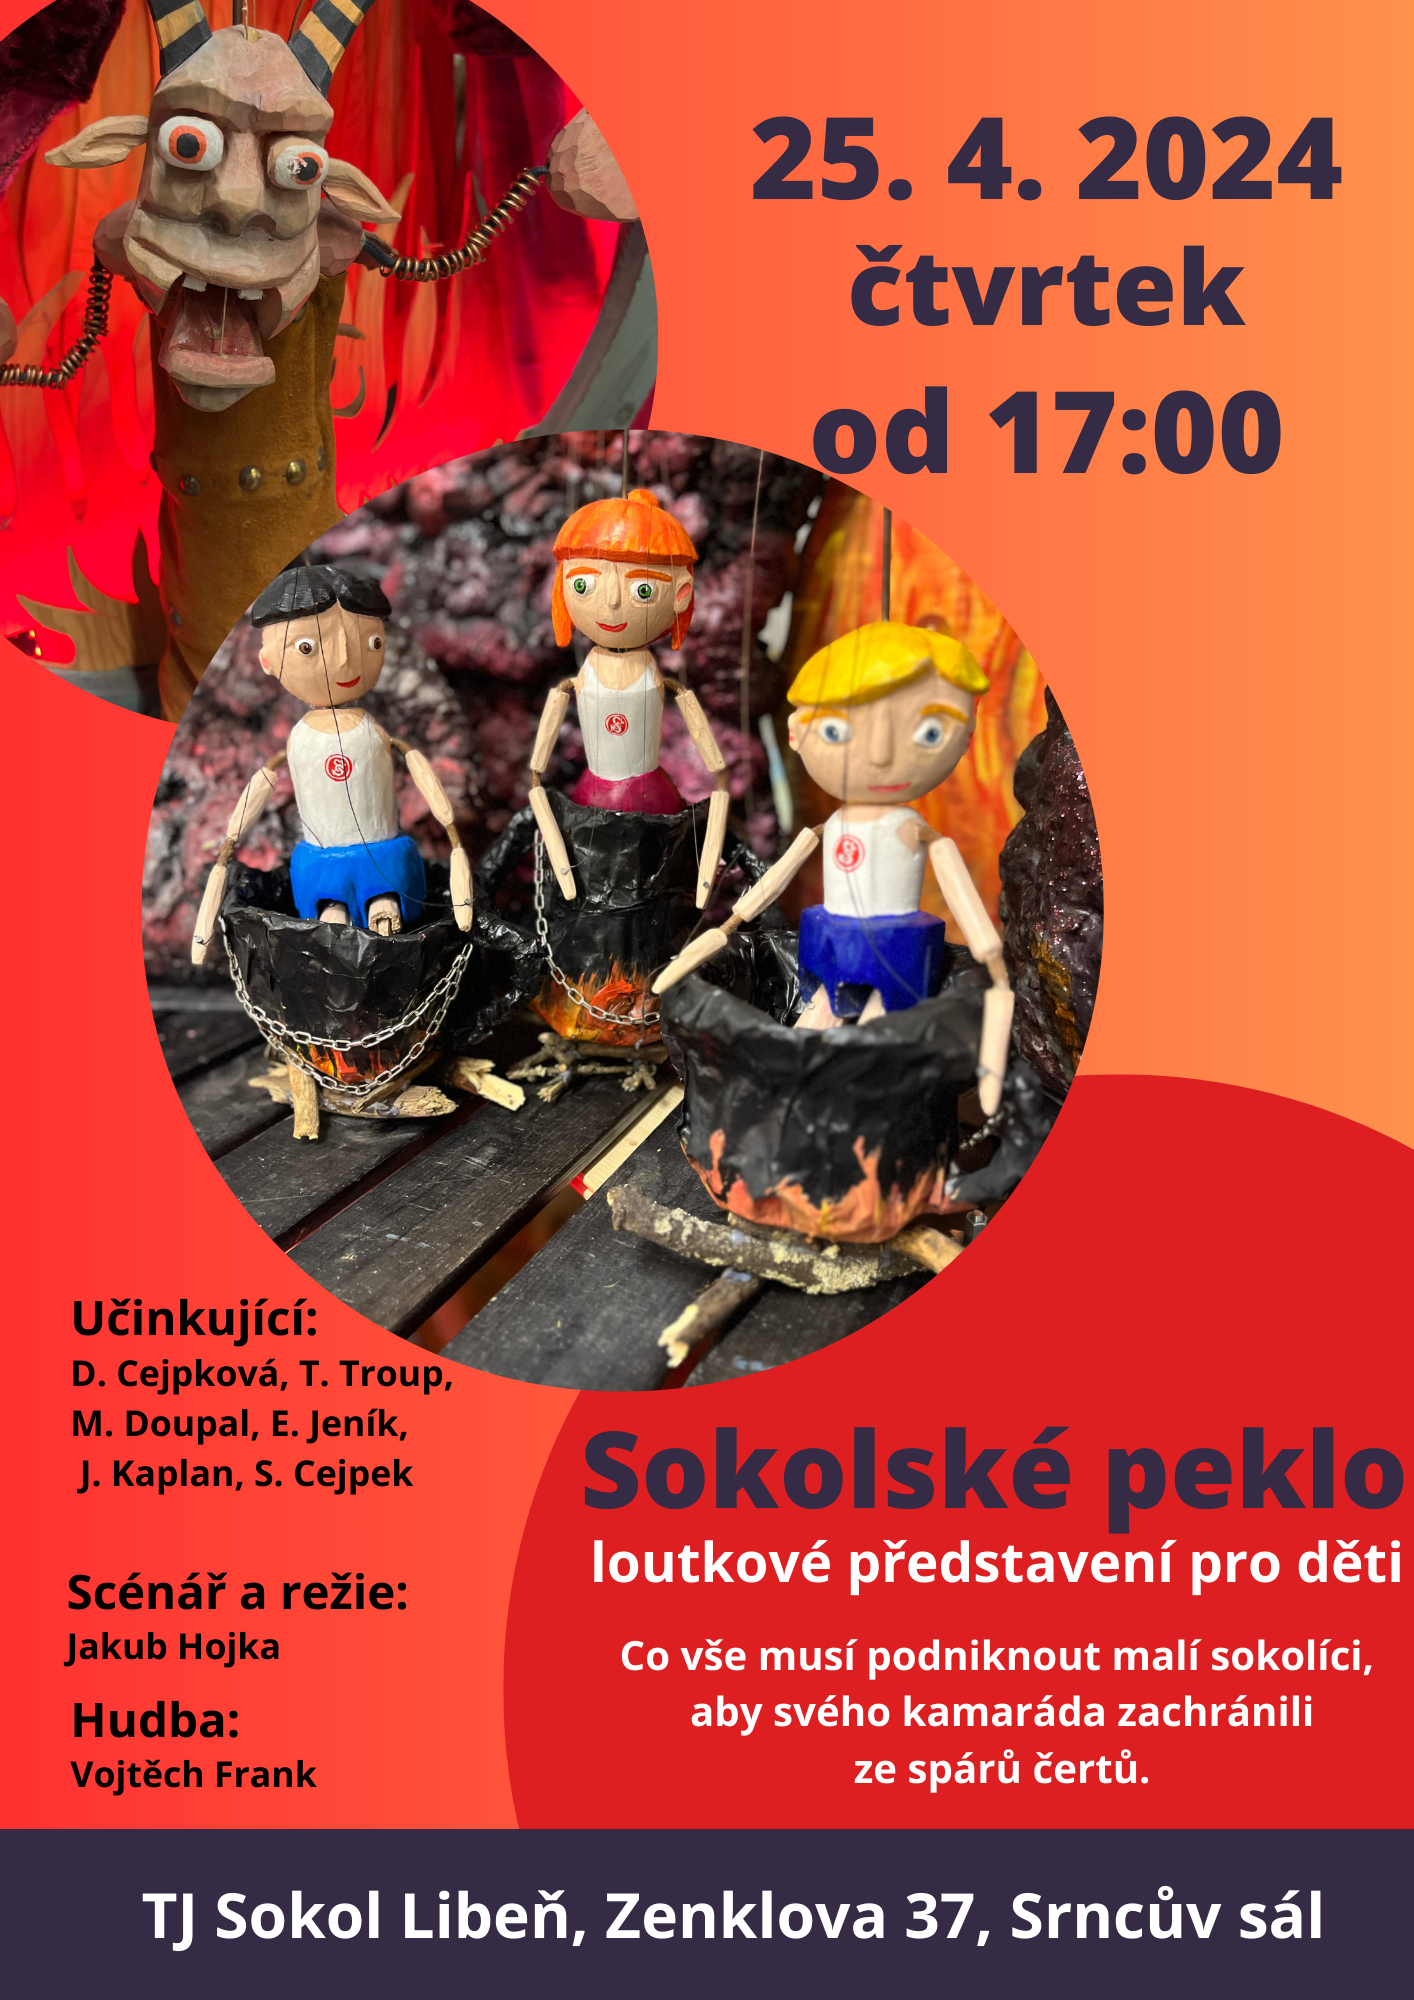
\includegraphics[width=\linewidth]{Sokolske_peklo_oprava.png}
\end{center}
\restoregeometry

\clearpage
\pagestyle{standard}

\post{Předškolní děti}
Ve druhém pololetí bude výuka v~hodinách předškolních dětí zaměřena na základy gymnastiky a atletiky. Vše souvisí s~plánovanými závody.

Dne \textbf{6. 4.} čekají vybrané děti závody v~gymnastice v~TJ Sokol Vršovice. Pravidelná příprava na závody probíhá v~pátek od 16:00 do 17:00. Držte nám palce, ať v~silné konkurenci obstojíme. 

Od \textbf{15. 4. budeme chodit cvičit s~dětmi ven} na doskočiště, abychom důkladně natrénovali skok do dálky a běh v~dráze, protože nás čekají v~květnu závody v~atletice. Děti budou přicházet do svých šaten, z~kterých budeme chodit na venkovní sportoviště, které je hned vedle sokolovny.

Opět bude v~létě probíhat \textbf{tábor pro předškolní děti a mladší školní děti} a to v~termínu 6.–13. 7. 2024. Tábor bude v~Janských Lázních v~Hotelu Večernice. Cena tábora je 6 200\,Kč. Na tábor můžete čerpat příspěvky svých zaměstnavatelů, pojišťoven či jiných neziskových programů. Pokud byste měli zájem dítě na tábor vyslat a brání Vám v~tom finanční situace, tak se obraťte na vedoucí cvičení, která Vám ráda poradí, kde o~příspěvek požádat.

Stále máme na cvičení hodně děti a zájem o~místa na školní rok 2024/25 už je nyní velký a přesahuje kapacitu oddílu. Další děti nemůžeme přijmout, protože nemáme dostatek cvičitelů, kteří by se mohli dětem věnovat. Pokud tedy máte zájem se zapojit více do chodu libeňského Sokola v~roli pomahatele či cvičitele, tak stačí kontaktovat jen vedoucí cvičení a říci si, jaké jsou Vaše představy a časové možnosti, jak se do činnosti organizace zapojit.

Rok 2024 je sletovým rokem, kdy Libeň bude mít na ploše nejvíce cvičenců z~celé České republiky ve skladbě Mravenci, proto také do naší jednoty zavítala Česká televize, která o~nácviku natočila krátkou reportáž do Sokolského zpravodaje.

\signature{Dana Cejpková}{tel.: 606 551 223\\e-mail: cejpkova.dana@seznam.cz}

\vspace*{24pt}

\clearpage

\newgeometry{margin=0pt}
\pagestyle{blank}
\begin{center}
  \noindent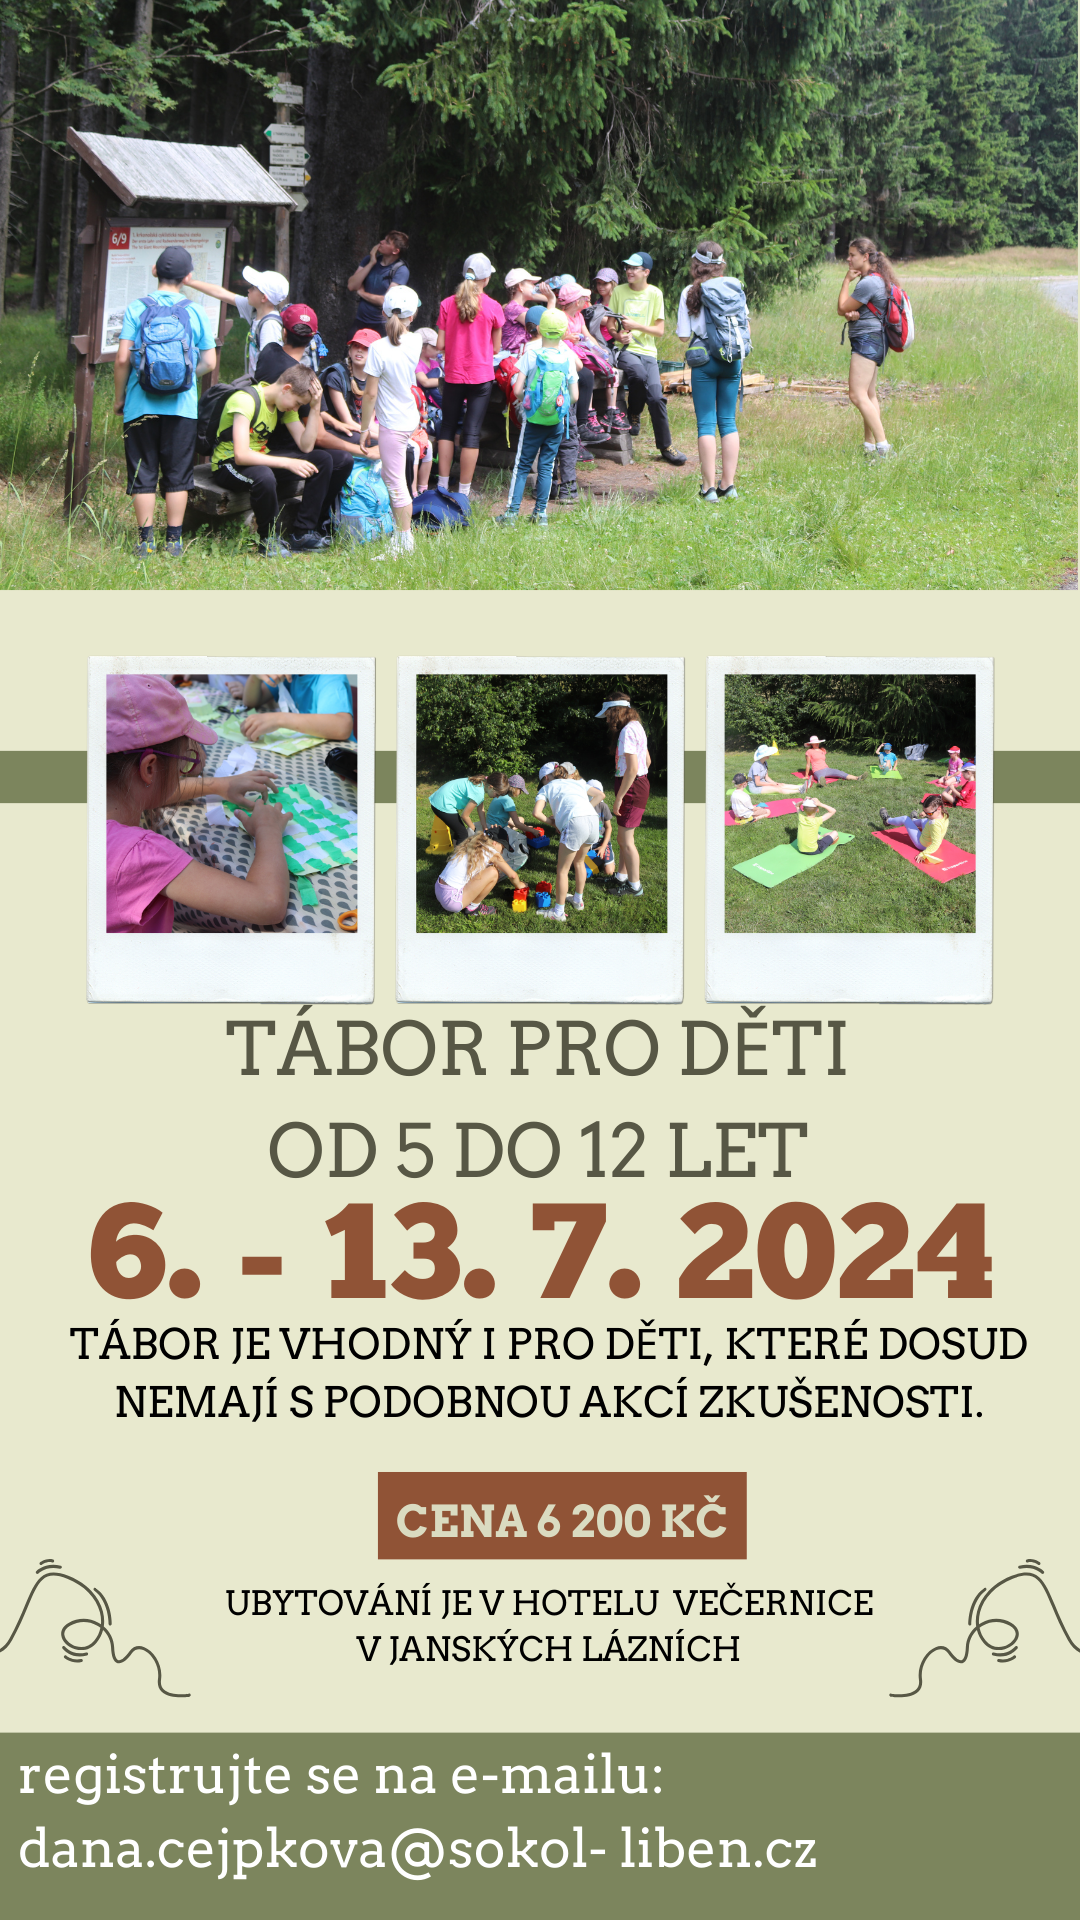
\includegraphics[height=210mm]{tabor_pd_2024.png}
\end{center}
\restoregeometry

\clearpage
\pagestyle{standard}

\post{Oddíl rodičů a dětí}
Na cvičení je stále velká účast, a tak určitě všechny potěší, že od pondělí 15. 4. bude probíhat cvičení jen na velkém sále, protože předškolní děti budou cvičit venku. Pokud by však odpoledne pršelo a předškolní děti by nemohly cvičit venku, tak se budou rodiče a děti automaticky přesouvat do Srncova sálu (ten se zelenou podlahou).

Časy hodin a jejich vedoucí se nebudou měnit ani v~následujících měsících:

\vspace*{6pt}
pondělí 16:00–17:00 Dana Cejpková

úterý 9:50–10:50 Jana Motlová

čtvrtek 16:00–17:00 Jana Dubská
\vspace*{6pt}

Prosím, začněte přemýšlet, jak budete chtít docházet na cvičení od září 2024. Už nyní je dlouhý seznam zájemců o~cvičení ve školním roce 2024/25. Dotazník týkající se Vašeho zájmu o~cvičení Vám přijde na konci dubna na e-mail.

Pod vedením Martiny Škochové oddíl pilně nacvičuje na slet skladbu Čmeláci. Podařilo se obsadit značky v~celém celku, takže nacvičuje 16 párů. 

Moc Martině děkujeme za její trpělivost s~rodiči, protože s~těmi je to často náročnější než s~dětmi.

\signature{Dana Cejpková}{tel.: 606 551 223\\e-mail: cejpkova.dana@seznam.cz}

\vspace*{24pt}

\post{Tančírna}
Po delší pauze se 24. února opět koná v~libeňské sokolovně taneční večer, máte-li zájem zopakovat si před šibřinkami pár tanečních kroků, dorazte a vezměte s~sebou i něco dobrého k~snědku, anebo příspěvek 50 Kč na občerstvení. Vítány jsou páry i jednotlivci, začínáme ve 20:00 v~Strnadově sále.

\vspace*{24pt}

\clearpage

\newgeometry{margin=0pt}
\pagestyle{blank}
\begin{center}
  \noindent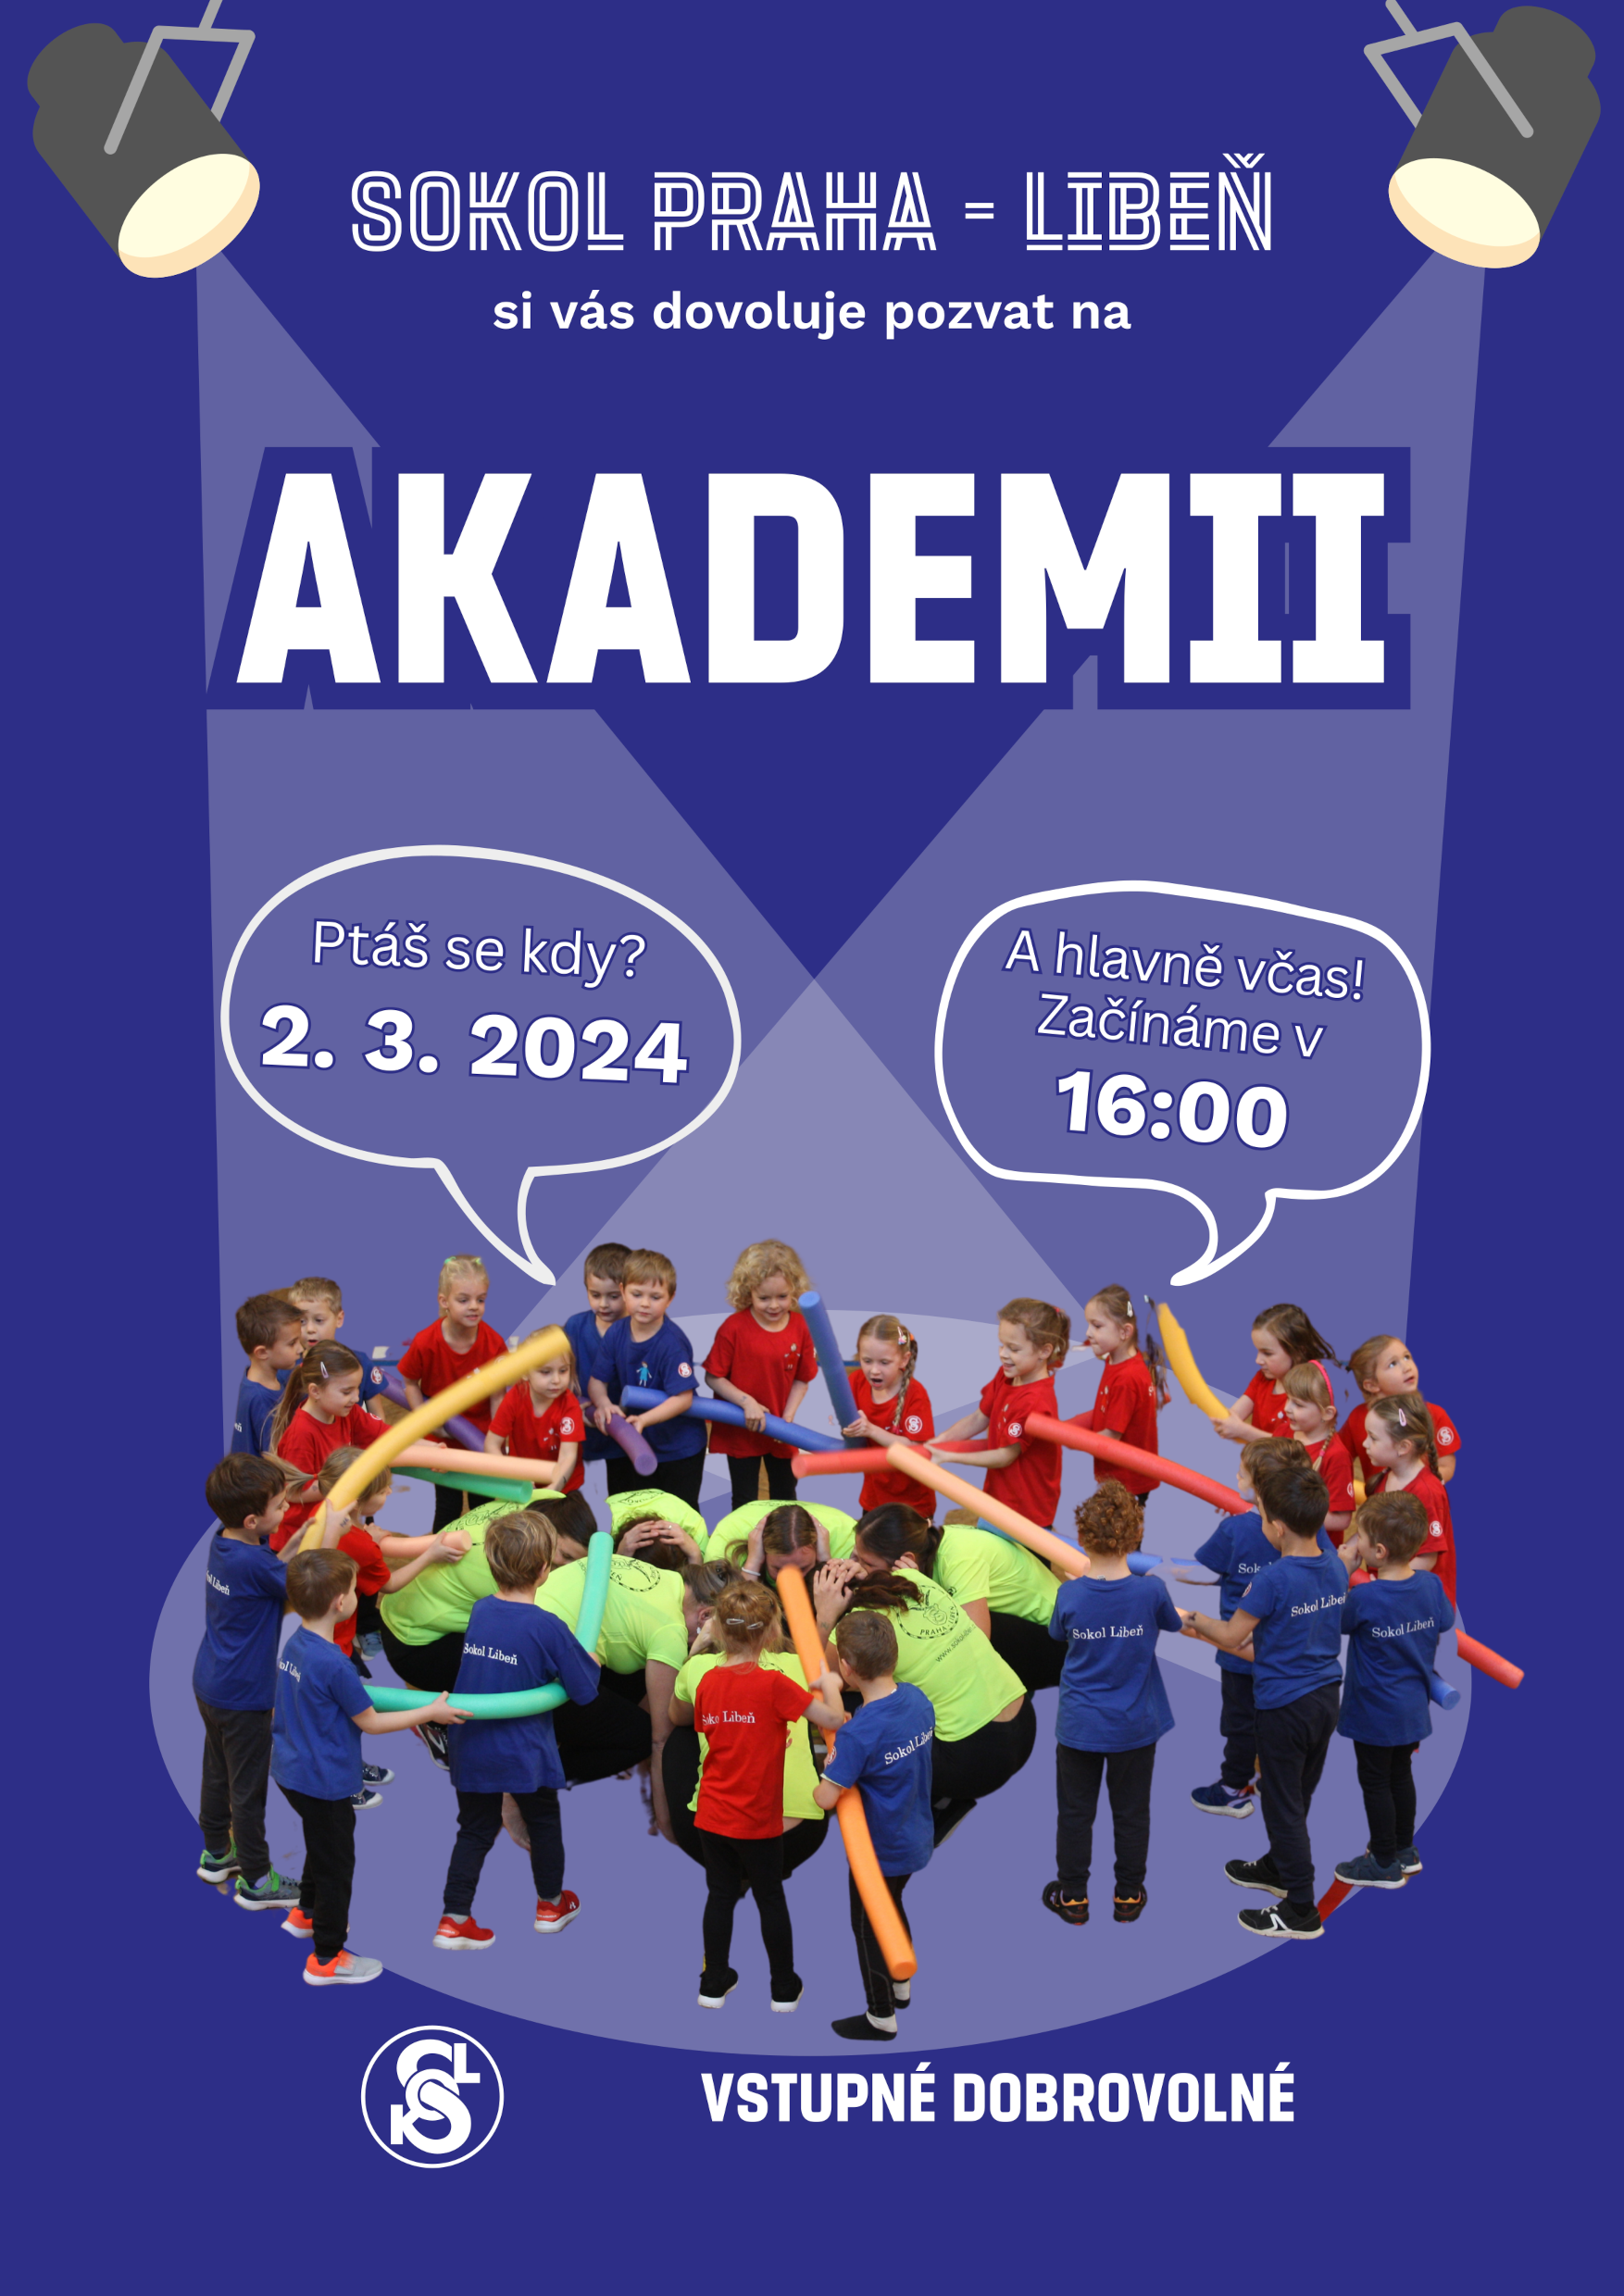
\includegraphics[width=\linewidth]{Akademie_24.pdf}
\end{center}
\restoregeometry

\clearpage
\pagestyle{standard}

\post{Ženy – všestrannost}
Nácviky na slet, přípravy na březnovou akademii a bohužel i různá zdravotní omezení se podepisují i na chodu oddílu Ženy-všestrannost, v~současné době se proto na běžném pondělním a čtvrtečním cvičení scházíme ve skrovnějším počtu. Přesto panuje v~oddíle dobrá nálada a kromě protaženého těla si z~hodiny zpravidla odnášíme i úsměv na tváři. Snad nám vydrží i v~dalších měsících, plných nejen sokolského ruchu.   

Za libeňské všestraňačky

\signature{Dubina}{}

\vspace*{24pt}

\post{Sokolská kapka krve}
V~lednu 2024 započal 10. ročník projektu. Nicméně, před pohledem do budoucnosti musíme nejprve zhodnotit ročník 9.

V roce 2023 se projektu Sokolská kapka krve zúčastnilo celkem 61 jednot a v nich 354 dárců absolvovalo 992 odběrů (v roce 2022 to bylo 860 odběrů). Loni tak sokolové darovali 446 litrů krve.

Vítěz je opět stejný jako vždy před tím. Stal se jím Sokol Komárov, který letos překonal opět sám sebe a 38 dárců absolvovalo 183 odběrů (v~loňském roce 2022 to bylo 108 odběrů).

Na 2. místě skončil Domašín a třetí je jednota z~Jihlavy. Další skvělé výsledky pak přišly ze Spořilova, Opočna či Krásné Hory nad Vltavou: všechno jednoty, které se účastní již opakovaně.

Letos se podařilo oslovit 66 prvodárců, což je v~době, kdy dle Českého červeného kříže v~Česku chybí asi 70 000 dárců, obzvlášť důležitý počin. 

K~podpoře a propagaci dárcovství pořádají sokolské jednoty i hromadné společné odběry: opakovaně v~Tyršově domě, ale i jinde.

Poslední hromadný odběr v~Tyršově domě se konal 16. 2. u~příležitosti výročního dne založení Sokola a odebráno bylo přes 60 dárců. 

V~roce 2023 v~Sokole Libeň krev darovali: Z. Burianová, M. Burian, F. Dostál, T. Dragoun, M. Frost, V. Jakoubek, M. Kubů, J. Kubišta a L. Zubáková. Celkem absolvovali 23 odběrů (o~9 více než v~r. 2022) a naše jednota se umístila na 12. místě. Podrobné výsledky jsou vyvěšeny na webových stránkách jednoty. 

Darovaná krev může pomoci v~mnoha situacích ohrožujících život: malým miminkům, maminkám po porodu, dětem i dospělým s~leukémií nebo obětem automobilových nehod či přírodních katastrof.

Veškeré informace o~projektu a plánovaných hromadných odběrech najdete na sokolskakapkakrve.cz.
Bližší informace také rád sdělím osobně či na e-mailu: vit.jakoubek@sokol-liben.cz.

Kdo v~Sokole Libeň darujete krev, pošlete mi prosím počet odběrů za 1. pololetí 2024 na výše uvedený e-mail do 31. 7. 2024.

Zkusme vystoupit ze své komfortní zóny, a pokud splníme podmínky pro darování krve a jsme zdrávi, pak bychom si odběr měli alespoň vyzkoušet. Mysleme na to, že darovaná krev může zachránit lidský život a to přece stojí za nějaké nepohodlí a námahu. 

\signature{Vít Jakoubek}{zdravotník jednoty}

{\color{sokolred}[fotka]}
\clearpage

\post{Se Sokolem do divadla}
Chladnější období k~návštěvě divadla a dalších kulturních institucí přímo vybízí, takže rubrika \luv{}Se Sokolem do divadla\ruv{} rozhodně netrpí okurkovou sezónou\,\dots{}

Posledním kulturním počinem, o~kterém jsem Vás informoval koncem roku, byla společná návštěva operety Polská krev českého skladatele Oskara Nedbala v~podání studentů pražské konzervatoře. Mimořádně vydařená derniéra této světoznámé a nejhranější české operety oslovila dokonce i dětské diváky. Děti jsou totiž ve svých reakcích většinou bezprostřední a v~kritice neúprosné. I~když jsme na představení odcházeli s~očima navrch hlavy a se slovy \luv{}proč zrovna opereta/zase nějaké zpívání/furt nějaké divadlo\ruv{}, bylo hned po několika minutách hravé a melodické hudby a salvách dětského smíchu jasné, že to byla \luv{}zase trefa do černého\ruv{}. A~když jsme se vraceli domů v~doprovodu běžných témat \luv{}bez puberťáckých komentářů a celkového rozladění\ruv{}, došli jsme k~závěru, že se opereta musela opravdu líbit! Věřím, že stejně jako mě zaujalo provedení Polské krve i ostatních 23 diváků z~řad Sokola Libeň.

Je mnoho věcí, které jsou tak říkajíc \luv{}mezi nebem a zemí\ruv{} v~běžném životě, v~divadle to je \luv{}Láska mezi nebem a zemí\ruv{}, kterou v~rámci nabídky \luv{}Se Sokolem do divadla\ruv{} 17. ledna 2024, jako první představení letošního roku, navštívilo 14 diváků. Všem zúčastněným se tato komedie \luv{}ze života\ruv{} v~podání amatérského divadelního souboru Bez dozoru líbila.

Hned dva dny poté, v~pátek 19. ledna 2024, se 11 posluchačů (z~celkem 13 přihlášených) nechalo v~majestátních prostorách Rudolfina v~rámci vzdělávacího cyklu vtáhnout do tajů italské hudby. Pod názvem \luv{}Bella Italia!\ruv{} nám moderátor Petr Kadlec a dirigent české filharmonie Marco Ivanovič za doprovodu studentské filharmonie přiblížili vybraná díla italských skladatelů.

Zatím poslední naše návštěva mířila do Divadla pod Palmovkou, kde celkem 20 \luv{}Libeňáků\ruv{} zhlédlo klasické představení Jiráskovy Lucerny v~podání sokolského divadelního souboru \luv{}Divadlo pod Petřínem\ruv{} v~režii Bohumila Gondíka. Jednalo se o~premiéru představení ku příležitosti blížícího se všesokolského sletu. I~toto představení jsme zhodnotili jako mimořádně vydařené a shodli jsme se, že Sokolové, kteří budou mít příležitost se na toto ztvárnění Lucerny podívat v~Národním divadle v~hlavním sletovém týdnu, se mají na co těšit.

Neváhejte a připojte se k~nám v~naší cestě za kulturou. Rádi Vás vezmeme s~sebou! A~pokud byste měli zajímavý tip na jakýkoli kulturní počin, podělte se o~něj a pošlete jej na e-mail zde níže.

\signature{Miloslav Doupal}{e-mail: mila.doupal@sokol-liben.cz}


\vspace*{24pt}

\post{Turistický oddíl JILM a Veverky}
Na úvod vítám všechny do nového roku a přicházím s~novinkami z~oddílu. Náplň schůzek se snažíme udělat co nejvíc různorodou a dostatečně stimulující mozkové buňky. Na schůzkách nechybí zábavné hry, písničky, STUZ (signalizace, topografie, uzly a zdravověda) nebo složitější program pro starší členy. Těší nás hojná účast na akcích (průměrně 18) a pozitivní ohlasy od členů. V~docházce máme zapsaných celkem 25 členů.

\vspace*{12pt}\noindent
Akce minulé:
\begin{itemize}[
  itemsep=-3pt,
  leftmargin=2em,
  itemindent=-1em
]
  \item[] 16.–17. 12. se vypravilo 18 členů a 4 vedoucí na Vánoční výpravu do zimní Plzně a okolí, kde jsme navštívili muzeum v~Horní Bříze a vydali se po stopách fazolového vraha.
  \item[] 20. 12. se v~klubovně pořádala Vánoční nadílka, kam přišlo 35 osob (18 členů, 5 vedoucích a 12 hostů z~řad bývalých členů). Ve vánoční atmosféře se zpívaly koledy, vzpomínalo na uplynulý rok a nakonec se i rozdaly dárky.
  \item[] 12.–13. 1. jsme páteční odpoledne strávili v~lezeckém centru Smíchoff s~bývalou vedoucí Kaktus a večer nás v~sokolovně pobavil film Rozpuštěný a vypuštěný. Celé akce se účastnilo 19 členů a 4 vedoucí.
  \item[] 1.–4. 2. (čt–ne) jsme v~počtu 18 členů a 5 vedoucích vyrazili na lyže na Ledňáčkovu chatu, v~programu nechybělo lyžování, Náčelník ztratil mokasín a jiné hry. Důležitou událostí pro členy byl vstup do služeb c. k. policejního ředitelství.
\end{itemize}

\clearpage
\vspace*{6pt}
\noindent
Akce budoucí:
\begin{itemize}[
  itemsep=-3pt,
  leftmargin=2em,
  itemindent=-1em
]
  \item[] 3. 3. (ne) Brigáda
  \item[] 16.–17. 3. (so–ne) Aprílovka
  \item[] 3. 4. (st) Mistr signalizace
  \item[] 13.–14. 4. (so–ne) JVLS a semifinále ZZZ
  \item[] 17. 4. (st) Mistr uzlování
  \item[] 10.–12. 5. (pá–ne) Finále ZZZ v~Úpici – pro trojky a náhradníky, kteří postoupí v~semifinále
  \item[] 31. 5.–2. 6. (pá–ne) Loďovka
  \item[] 21. 6.–23. 6. (pá–ne) Pracovka – povinná pro všechny účastníky tábora
  \item[] 19. 7.–21. 7. (pá–ne) Stavba tábora – pro děti nepovinná, ale každá pomoc vítaná
  \item[] 10.–31. 8. Tábor
\end{itemize}

\noindent
Pokud máte jakékoliv dotazy, připomínky nebo nápady, neváhejte se obrátit na náš e-mail: jilmveverky@sokol-liben.cz

Za společný oddíl
 
\signature{Bára Jeníková}{}


\post{Šibřinky 2024}

Přijďte oprášit své taneční kreace a staré sletové úbory na tradiční libeňské šibřinky s~podtitulem Sletu zdar!

\noindent
Co vás čeká:

Přátelská atmosféra 

K~tanci i poslechu živá kapela 

Pestrý program a tombola

\noindent Datum: 23. března

\noindent Čas: 19:00 

Příspěvek na organizaci akce a kapelu 250 Kč předem případně 300 na místě.

Přijďte s~přáteli a rodinou strávit večer plný smíchu, tance a nezapomenutelných chvil! Označte si datum v~kalendáři a dejte nám vědět, jestli se k~nám přidáte. Těšíme se na vás!

\clearpage

\pagestyle{blank}
\newgeometry{margin=1cm}

\vspace*{96pt}

\pagecolor{sokolred}
\color{white}

\noindent {\fontsize{48pt}{56pt}\tyrs
se sokolským

\vspace*{24pt}

\noindent nazdar!}

\vspace*{\fill}

% \color{black}
\begin{center}
Vydává Tělocvičná jednota Sokol Libeň, Zenklova 37, Praha 8

\vspace*{12pt}

Na přípravě tohoto čísla se spolu s~autory jednotlivých textů podíleli:

grafická úprava – Martin Burian | jazyková úprava – Martina Waclawičová \\ editoři textů – Vít Jakoubek, Jan Přech
\end{center}

\end{document}